\documentclass[12pt]{article}
\usepackage{fancyhdr}
\usepackage{lastpage}
\usepackage{geometry}
\usepackage{amsmath}
\usepackage{setspace}
\usepackage{graphicx}
\usepackage{caption}
\geometry{a4paper,scale=0.8}
\pagestyle{fancy}
\lhead{Team 1}
\rhead{April 17th, 2019}
\chead{Project Report}
\cfoot{page \thepage \  of \pageref{LastPage} }
\renewcommand{\headrulewidth}{0.4pt}
\renewcommand{\footrulewidth}{0.4pt}
\setlength{\baselineskip}{23pt}
\begin{document}
		\section{Abstract} % Numbered section
	
	This paper performs a validity test of Fama French three-factor model on the stocks listed in NYSE, NASDAQ and AMEX, i.e. US markets, using period spanning from Jul 2011 – Dec 2018. Monthly stock returns, and 1-month T-bill returns are collected over the period from Jul 2011 – Dec 2018 to construct the monthly excess returns for each of the stocks. The monthly excess returns suggest that larger-sized companies (i.e. Big-sized) have higher excess returns than portfolios containing smaller sized firms on an average. On the other hand, portfolio constructed of low book-to-market ratio firms look to perform better than those constructed of high book-to-market ratio firms. Quintiles of portfolios, i.e. twenty-five portfolios, are constructed in accordance to size and book-to-market ratio to help explain the variations on excess portfolio returns by using market risk factor, size risk factor and book-to-market ratio risk factors. After conducting some analysis and statistical tests, we have arrived at the conclusion that size factor has no effect on portfolios having big-size firms but can explain the excess return variations on portfolios having small and medium-sized firms. On the other hand, book-to-market ratio factor has an effect on portfolios with high book-to-market ratio firms. Therefore, we have concluded that Fama French model only has explanatory power over portfolios of several characteristics, but do not help to explain the whole market as a whole during the period spanning from Jul 2011 – Dec 2018.
	
	
	\section{Introduction} % Numbered section
	
	The emergence of Modern Portfolio Theory by Markowitz (1952) has set the foundation for portfolio management research, and at the same time incited several research papers with such focus, like Capital Asset Pricing Model (CAPM) developed by Sharpe (1964) and Lintner (1965). Citing CAPM as an example, it aims to explain the stock returns using excess market returns as the only risk factor by using the covariance of portfolio returns with the market portfolio return to explain the variations in each of the portfolio excess returns. However, Fama and French think otherwise and proceeded to prove that covariance has little or no power in terms of explaining cross-sectional variations in equity returns. \\
	
	\noindent Therefore, Fama and French set this as a motivation, and proceeded to add in another two more risk factors, i.e. difference in the excess returns between Small and Big market capitalization sizes (SMB, Small Minus Big) and difference in the excess returns between High and Low book-to-market (High Minus Low, HML), in the original CAPM hoping to help address any initial anomalies introduced by the former. The results of this paper are encouraging as it proves that Fama and French 3 factor model has much higher explanatory power than the CAPM model but there still exists several drawbacks. The below displays the Fama and French model: \\
	
	\noindent $R(t) - R_f(t) = a+ b(R_{mkt} - R_f) + s(SMB) + h(HML) +\epsilon_i$ \\
	
	
	\noindent In recent times, there have been several motivations to add other risk factors into the original Fama and French model, which Fama and French extending the model by suggested profitability, i.e. RMW (Robust Minus Weak), and investment, i.e. CMA (Conservative Minus Aggressiveness). In addition, there have been several calls by the market to add in risk factors such as momentum and low-volatility as part of the model. \\
	
	\noindent Therefore, we are inspired to prove that the Fama and French 3 factors doesn’t help to explain the excess returns in the modern days, i.e. from Jul 2011 – Dec 2018, as well, and further encourages us to extend the original 3 factor Fama French Model; Furthermore, we have proceeded to setup the following hypothesis for our research purpose: {\textit{The three stock-market factors suggested by Eugene F. Fama and Kenneth R. French in their 1993 paper titled “Common Risk Factors in the Returns on Stocks and Bonds” do not significantly explain the returns of stocks listed on the NYSE, NASDAQ and AMEX for the period between Jul 2011 – Dec 2018.}}
	
	
	\section{Literature Review} % Numbered section
	
	The three-factor model introduced by Fama and French (1993) has come a long way in shaping views about drivers of stock returns in academia and in practice. On top of the market $\beta$ factor proposed and popularised by Sharpe (1964), Lintner (1965) and Black (1972) in their Capital Asset Pricing Model (CAPM), Fama and French (1993) proposed two additional and empirically-backed factors for the explanation of stock returns: Size (ME) and Book-to-Market Equity (BE/ME). \\
	
	\noindent The three-factor model was proposed in response to several discovered empirical contradictions to the CAPM highlighted in Fama and French (1992a). For one, Banz (1981) found that Size (proxied by Market Equity, or ME) adds explanatory power to cross-sectional average returns provided by market $\beta$s. Also, Bhandari (1988) found a positive relationship between firm leverage and average stock returns. To add, Rosenberg, Reid and Lanstein (1985) and Stattman (1980) discovered a positive relationship between Book-to-Market Equity and average U.S. stock returns. Further, Basu (1983) found that earning-price ratios (E/P) help in the explanation of cross-sectional U.S. stock returns when used in conjunction with size and market $\beta$ factors. These findings contradict the viewpoint that market $\beta$s alone are sufficient in describing cross-sectional expected stock returns. \\
	
	\noindent Amongst the potential and empirically-backed factors for stock returns mentioned earlier, Fama and French (1992a) found that Size (ME) and Book-to-Market (BE/ME), when used together, appear to absorb the roles played by leverage and E/P as explanatory factors for stock returns. it was also discovered that Size and Book-to-Market are able to well-explain cross-sectional average returns for stocks listed on the NYSE, Amex and NASDAQ for the period between 1963 to 1990. This discovery laid the groundwork for the three-factor model proposed by Fama and French (1993).\\
	
	\noindent In their study, Fama and French (1993) divided eligible common stocks traded on the NYSE, Amex or NASDAQ into six portfolios based on their Size and Book-to-Market Equity. Size was proxied by Market Equity (ME), and stocks were determined to be Big (B) or Small (S) based on whether they were above or below the median NYSE ME. Stocks were also determined to have Low (L), Medium (M) or High (H) Book-to-Market Equity based on whether they belonged to the bottom 30\%, middle 40\% or top 30\% of NYSE BE/ME. The resulting six portfolios formed were: S/L, S/M, S/H, B/L, B/M and B/H. Monthly Size (SMB) and Book-to-Market Equity (HML) factor readings were then constructed from the returns of these six portfolios. The Market factor was proxied by $R_M - R_F$, where $R_M$ is the result of the value-weighted return of eligible common stocks and $R_F$ is the one-month U.S. Treasury bill rate. Data relating to the study were obtained from the CRSP and COMPUSTAT.\\
	
	\noindent Fama and French (1993) then proceeded to use the same eligible stocks (used in the SMB and HML factor constructions) to construct 25 portfolios based on their Size and Book-to-Market Equity quintiles. The monthly excess returns of these 25 portfolios were then used as the dependent variables for regressions against the Market, Size and Book-to-Equity factors (the independent variables). It was found that, when used together, the three stock market factors were able to explain most of the variation in the returns of the 25 portfolios.\\
	
	\noindent It was also found that the SMB slope coefficients decreased monotonically as portfolio Size increased, whilst the HML slope coefficients increased monotonically as portfolio Book-to-Market Equity increased. Further, the regression intercepts were found to be mostly statistically indifferent from zero. On the other hand, when the Market factor was the only independent variable in the regressions, lower $R^2$ values were obtained and the Size effect seen in the intercepts discovered by Banz (1981) appeared. Overall, the results of the study offered compelling evidence in support of Size and Book-to-Market Equity as additional explanatory factors for stock returns.\\
	
	\noindent With all that said, the three-factor model is not without its criticisms. For instance, Daniel and Titman (1997) argued that it is the firm characteristics (e.g. region, industry, related lines of business etc), not the covariance structure of returns that actually explain the cross-sectional variation in stock returns. Daniel and Titman (1997) discovered that, once firm
	characteristics were controlled for, expected returns did not seem to be positively related to Market, SMB and HML loadings. The study was conducted for returns over 20.5 years between July 1973 to December 1993. Davis, Fama and French (2000), however, rebutted with their own findings with a higher-powered test, owing to a longer test period of 68 years between July 1929 and June 1997.\\
	
	\noindent Further, a plethora of subsequent studies successfully replicating the insights obtained from Fama and French (1993) for different regions and for different time periods have lent further credence to the notion that the Size and Book-to-Market Equity factors are indeed viable additions to the Market factor as explainers of stock returns. We seek to be able to further support the notion for stocks traded on the NYSE, Amex and NASDAQ for the period between July 2011 and December 2018.\\
	
		
\section{Data}
\subsection{Research Sample}
\noindent Our data sample includes all the stocks listed on the NYSE, NASDAQ and AMEX for the period between July 2011 to December 2018.And we use monthly data to calculate return.
\subsection{Data Source: Warton Research Data Services(WRDS)}
Wharton Research Data Services (WRDS) provides the leading business intelligence, data analytics, and financial research platform to global institutions ̶ enabling comprehensive thought leadership, historical analysis, and insight into the latest innovations in academic research.\\
And WRDS provides us with the following sub-database which we can utilize:
\begin{itemize}
	\item Center for Research in Security Prices(CRSP)
	\item Compustat-Capital IQ
	\item CRSP/Compustat Merged(CCM)
\end{itemize}
\subsubsection{CRSP}
\noindent The Center for Research in Security Prices (CRSP) maintains the most comprehensive collection of security price, return, and volume data for the NYSE, AMEX and NASDAQ stock markets. Additional CRSP files provide stock indices, beta-based and cap-based portfolios, treasury bond and risk-free rates, mutual funds, and real estate data.\\

\noindent And what we need is the monthly closing stock price, number of shares outstanding and returns of all US stocks. We use PERMCO, PERMNO as identifiers when we extract data from the databases.
\subsubsection{Compustat}
\noindent We extract total stockholders' equity, deferred taxes, investment tax credit and preferred stock relevant information from this database. And further more we calculated Book Equity(BE) and Market Equity Value(ME) along with the BE/ME in this step. And we use GVKEY as the unique identifiers.
\subsubsection{CCM}
\noindent The official CRSP/Compustat Merged Database (CCM) is comprised of CRSP and Compustat data together with the link and link-history references between these two databases. It includes Standard \& Poor's Compustat data, reformatted into CRSP's propreitary CRSPAccess database format, plus additional data tables that map the CRSP permanent company and security identifiers (PERMCO and PERMNO, respectively) to the COMPUSTAT permanent company identifier (GVKEY).\\

\noindent A common misconception is that CCM is CRSP stock market data merged with Compustat accounting data. This is not the case. CCM contains only Compustat data items, but can be searched by CRSP's PERMNO and PERMCO in addition to Compustat's GVKEY. Merging this data with the CRSP stock data requires an additional step. So we use CCM to obtain entity level matching data, then raw data was obtained from standalone datasets. New identifier GVKEY PERMCO was created for purposes of traversing between datasets.
For example, if Apple Inc’s GVKEY is 1690 and its PERMCO is 7, its GV KEY PERMCO is 16907, which is a unique identifier.

\subsection{Factor construction}
$$
R_{i_t}-R_{f_t}=\alpha_{it}+b_{it}(R_{M_t}-R_{f_t})+s_{i_t}(SMB)+h_{i_t}(HML)+\epsilon_{i_t}
$$
\subsubsection{Rm-Rf}
The excess portfolio return in month t, $(R_{M_t}-R_{f_t})$, is the excess market portfolio return in month t. In this study, we construct our own market portfolio to estimate the market return.Additionally 1-month T-bill rates are used as a proxy for the risk free rate.
\subsubsection{SMB and HML}
\noindent For each month SMB is the difference between the average of the returns on the three small-stock portfolios (S/L, S/M and S/H) and the average of the returns on the three big stock portfolios (B/L, B/M and B/H).
$$
SMB=[(S/L+S/M+S/H)-(B/L+B/M+B/H)]/3
$$
HML is the difference between the average of the returns on the two high-BE/ME portfolios (S/H and B/H) and the average of the returns on the two low-BE/ME portfolios (S/L and B/L).
$$
HML = [(S/H+B/H)–(S/L+B/L)]/2
$$

\subsubsection{Regression variable generation: 25 portfolios' return}
After the construction of SMB and HML portfolios for independent regression variables, 25 portfolios are constructed with a similar procedure in order to calculate excess portfolio returns for each month. All  stocks used in the analysis are sorted by size and distributed into five groups (s1 to s5) such that each group contains the correspounding quantile portfolio's return respect to SIZE and s1 contains stocks with smallest market cap, s5 with the biggest ones. Moreover, stocks are independently allocated to another five groups (b1 to b5) based on the book-to-market equity (BE/ME). 25 portfolios are constructed as the intersection of the five size groups and five BE/ME groups. For example, s5/b1 portfolio is constructed by the stocks in the biggest fifth of firms and the lowest fifth of BE/ME ratio.

\subsection{Other Issues in Data}
\begin{itemize}
	\item Missing Data: E.g. No returns data available when it should be
	\item Incomplete Dataset: CRSP \& Compustat do not cover the whole population of NYSE, NASDAQ and Amex traded stocks, only an overlap is available
	\item Repeat Data: Double reporting of same company for same period
	\item Conflicting Data: Standalone CRSP \& Compustat vs. CCM
	\item Computational Cost: Takes hours to compute several million cells	
\end{itemize}
\newpage

\subsection{Final Data Demostration}
\begin{figure}[ht]
	\centering
	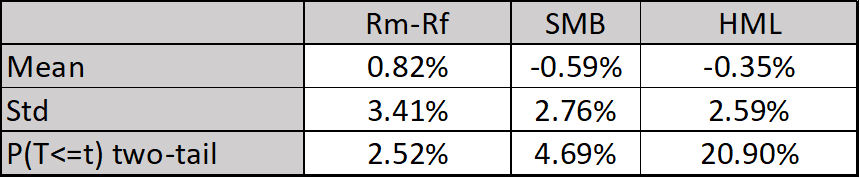
\includegraphics[scale=0.5]{1.png}
	\caption*{25 Portfolios}
	\label{fig:label}
\end{figure}
\begin{figure}[ht]
	\centering
	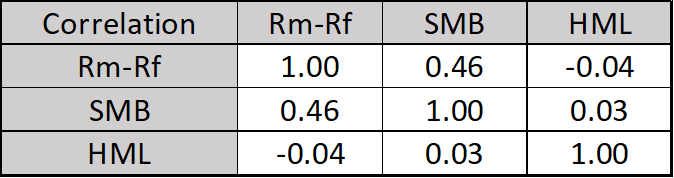
\includegraphics[scale=0.47]{2.png}
	\caption*{3 Factors}
	\label{fig:label}
\end{figure}


\section{Summary of Statistics}
\subsection{The explanatory variables}

The table below gives mean, standard deviation and test statistics for the three explanatory variables. The mean of market risk premium, 0.82\%, which implies 9.84\% on the annual basis, is much higher than what Fama and French reported (0.43\%) for their test period during 1963-1991. Both SMB and HML surprisingly turn negative with t-test suggests SMB is statistically significant from 0 with 95\% confidence level. In other words, small cap portfolios underperform large cap portfolios, high BE/ME portfolios no longer outperform low BE/ME portfolios. These are huge paradigm shift from Fama and French’s observation.

%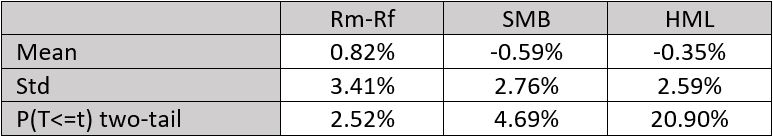
\includegraphics[scale=0.6]{1.JPG}

\begin{figure}[h]
	\centering
	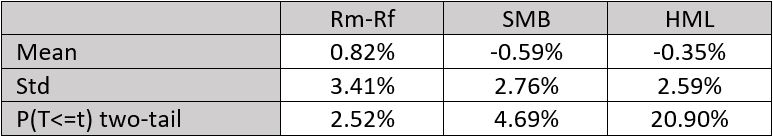
\includegraphics[width=0.5\linewidth]{1.JPG}
	\caption*{Table 1}
	\label{fig:label}
\end{figure}


\noindent The correlation matrix shows HML has little correlation with market risk premium and SMB. This implies HML brings in additional explanatory power that CAPM is not able to capture.

\begin{figure}[h]
	\centering
	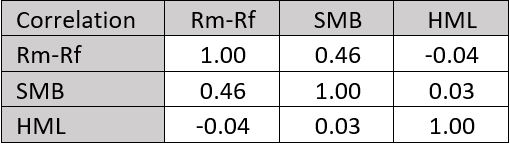
\includegraphics[width=0.35\linewidth]{2.JPG}
	\caption*{Table 2}
	\label{fig:label}
\end{figure}


\subsection{The dependent variables}   

Table below lists average of annual number of firms in each portfolio. 61.7\% of firms lie in the union of smallest cap quintile and lowest BE/ME quintiles (as highlighted).



\begin{figure}[h]
	\centering
	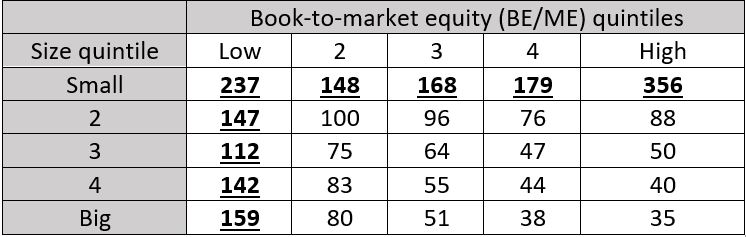
\includegraphics[width=0.5\linewidth]{3.JPG}
	\caption*{Table 3}
	\label{fig:label}
\end{figure}

\noindent Table 4 demonstrates average of monthly excess return for all 25 portfolios between 2011-2018. We are able to find a clear trend that excess returns get higher when size increase in each BE/ME quintiles. This finding aligns with the observation in Table 1. On the other hand, we can see lower BE/ME portfolios yields higher excess return in size quintiles “3” and “Big”, but the consistency does not hold for the other size quintiles. This inconsistency explains why the null hypothesis for HML in sections 1.1 was not rejected.

\begin{figure}[h]
	\centering
	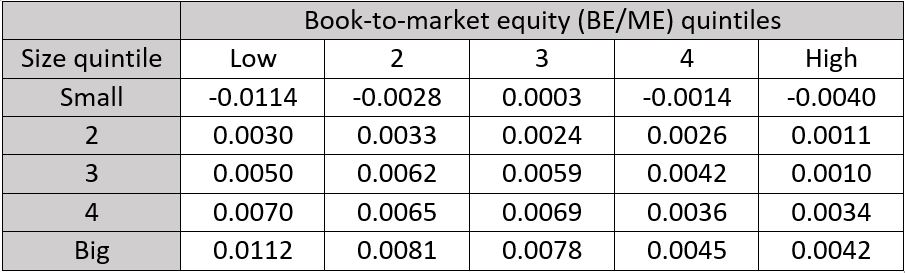
\includegraphics[width=0.55\linewidth]{4.JPG}
	\caption*{Table 4}
	\label{fig:label}
\end{figure}

\section{Time-series Regression Results}


After performing linear regression for 25 portfolios between 2011-2018, coefficients for all regressors have been summarized in Table 5. First of all, for intercept a, we are unable to reject null hypothesis in 24/25 portfolios, except for the portfolio on the upper left corner as highlighted. This is to convey there is no abnormal return in FF-3 factor model, which implies its capability in explaining stock return variation. Secondly, t-test results for slope b suggest rejection of null hypothesis. As anticipated, values of slope b are close to 1. Thirdly, t-statistics are strong enough to reject null hypothesis for s (slope for SMB) in four smaller size quintiles. The exception happens for “Big” size quintiles where slopes turn negative as highlighted. Similarly, for HML, t-tests are not able to reject null hypothesis when h turns into positive from lower BE/ME quintile to higher BE/ME quintile.

\begin{figure}[h]
	\centering
	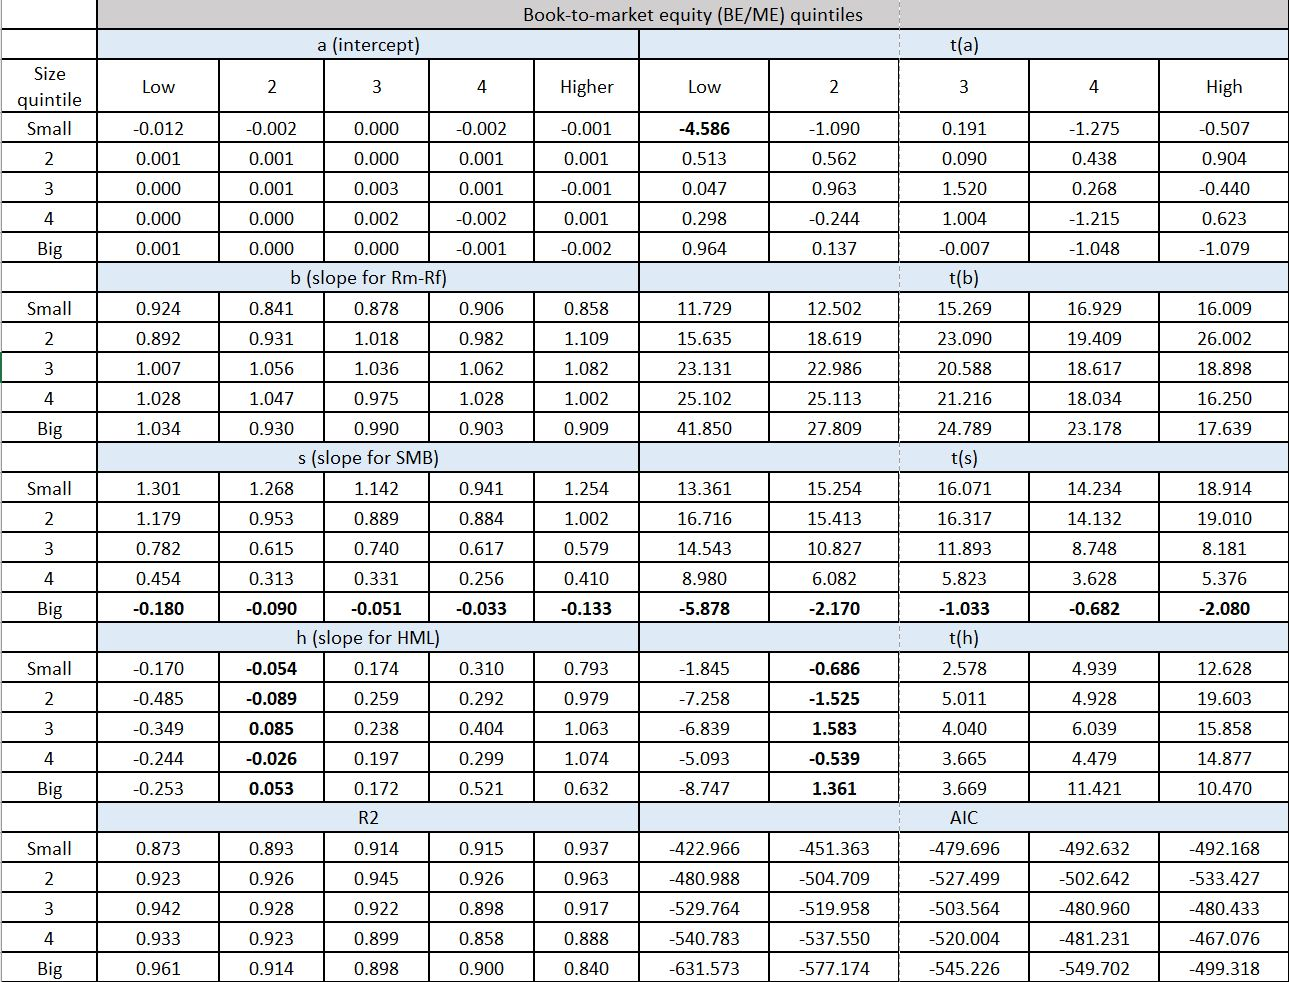
\includegraphics[width=1\linewidth]{5.JPG}
	\caption*{Table 5}
	\label{fig:label}
\end{figure}


\noindent In order to prove stronger explanatory power of FF-3 factor model, regression analysis has also been conducted on single factor CAPM. Results are tabulated below. Generally, t-statistics for intercept are much higher than they are in FF-3 in absolute term. This implies abnormal returns vanish with introduction of SMB and HML. On the other hand, b values for CAPM tend to be higher than when they are in FF-3. Last but not least, discrepancies of R2 in Table 5 and Table 6 indicate FF-3 factor model improves the explanatory power from 50\%-90\% range (CAPM) to 84\%-96\% range.



\begin{figure}[h]
	\centering
	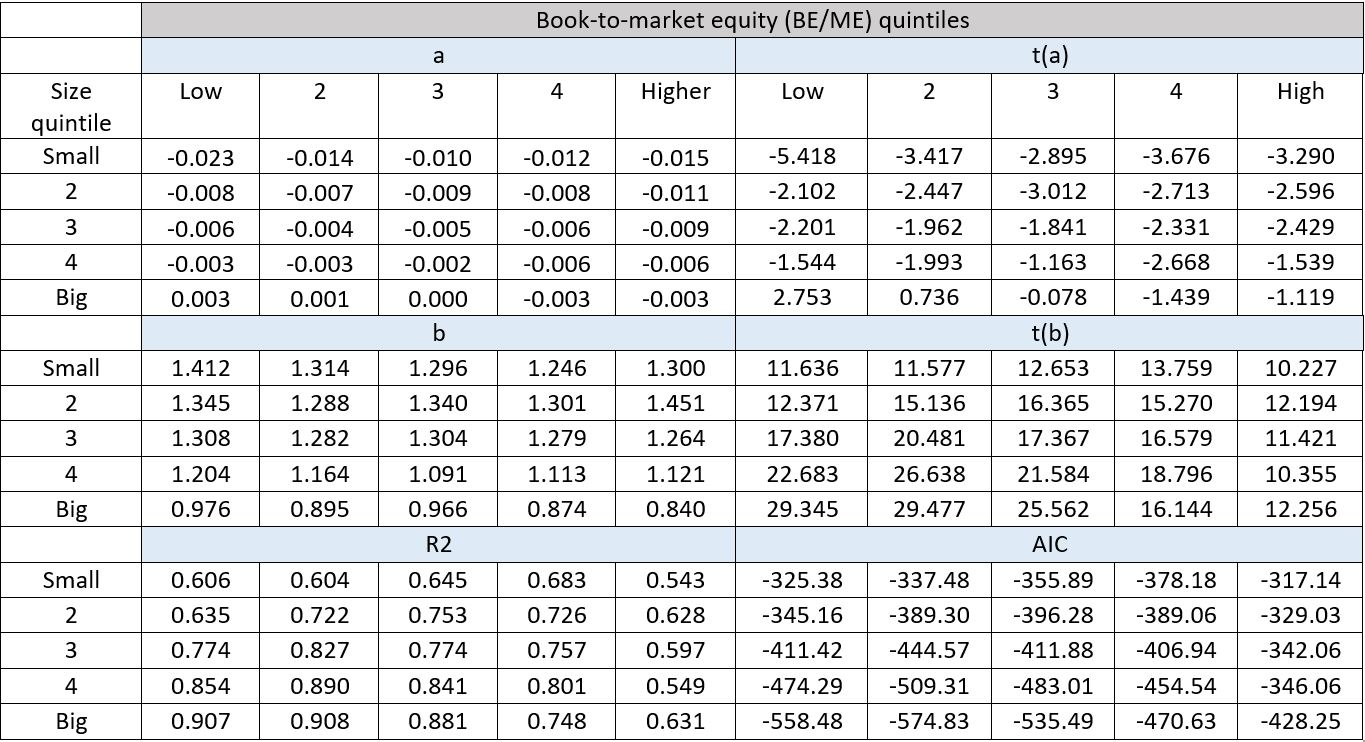
\includegraphics[width=1\linewidth]{6.JPG}
	\caption*{Table 6}
	\label{fig:label}
\end{figure}

\section{Interpretation}

Fama and French explained size and BE/ME are not ad hoc variables for explaining average stock return(1992b). They believe both variables are related to economic fundamentals. Firms that have high BE/ME ratio tend to have low earnings on assets. The intuition is that investors would not be attracted by firms that have poor earning performance recently. Reversely, investors tend to invest in firms with strong earning/profitability figure recently (1992b). Size is also related to profitability. Fama and French attributed size effect to smalls firms not able to participate in economic boom of the middle and late 1980s., which pushed small firms to a long earnings depression. However, their paper in 1992b and 1993 did not explain how size and BE/ME’s relationship with earning leads to their relationship with average excess returns (of 25 portfolios).
Practitioners have been debating on whether the outperformance tendency is due to market efficiency or inefficiency. The “inefficiency” proponents believe the outperformance is explained by incorrectly value pricing of companies by market participants. However, the “mispricing view” does not explain why small firms were mispriced higher instead of lower between 1963-1991. 
Given the paradigm shift mentioned in section 1.1 that small firms outperformed large firms between 2011-2018. We would like to vote for “efficiency”. Intuition comes as: in old days such as 1963-1991, it was not easy for investors to access to or liquidate small-cap stocks. In addition, small firms normally have higher cost of capital and greater business risk. All of these made small-cap stocks riskier to invest, hence higher return in old days. On the other hand, it is much easier for investors to access to small-cap stocks and liquidate nowadays. More transparent market also reduces risk of investing in small firms. These could explain why small cap stocks does not outperform large cap stocks as they used to be. However, more evidence needs to be found to support our intuition and more insight needs to be brought in in order to explain why small cap stocks underperform large cap stocks between 2011-2018.

	\section{Conclusion} % Numbered section
In conclusion, we have accomplished our research objective to prove that Fama and French three-factors model does not significantly explain the returns of stocks listed on the NYSE, NASDAQ and AMEX for the period between Jul 2011 – Dec 2018. Together with the market data collected from various sources and statistical significance tests performed, all quintiles, except for Big-Sized portfolios and Low Book-to-Market quintiles, are able to base on this model to explain their returns as seen in the high t-stat values results derived. Size factor, i.e. SMB, proves to be ineffective on Big-Sized portfolios, and the intuition, according to Fama and French, is that the small-cap companies tend to see higher returns than large-cap companies in the long run. On the other hand, Book-to-Market factor, i.e. HML, is found to have no effect on Low Book-to-Market quintiles, in which the intuition is that value companies (high book-to-market ratio) enjoy higher returns than growth companies (low book-to-market ratio) in the long run. Lastly, market risk factor seems to suggest as a significant factor for portfolio returns of all quintiles. Therefore, we can deduce that Fama and French three factor model does have some explanatory power over certain quintiles of certain characteristics but does not explain well for the whole market. \\


\noindent In recent times, research has also further encouraged the development of other risk factors such as low-volatility, and momentum risk factors; In order to fit the quintiles better in the future, we could add in more non-collinear risk factors into the original to help explain the returns of the quintiles better going forward. Several statistical techniques can be applied to accomplish that, and machine learning can also help to the discovery of new risk factors as well. However, that is to say that different markets have different characteristics, in which one market model cannot be applied to another.\\


\end{document}